\documentclass{article}
\usepackage[hidelinks]{hyperref}
\usepackage{graphicx}
\usepackage{amsfonts}
\usepackage{amsmath}
\usepackage{enumitem}
\usepackage{polski}
\usepackage[utf8]{inputenc}
\usepackage{indentfirst}
\usepackage{float}
\title{Dokumentacja projektu dotyczącego optymalnego układania klocków na planszy}
\author{Abdelkarim Ahmed, Cacko Agata, Hernik Aleksandra}
\begin{document}
\maketitle
\section{Opis projektu}
\section{Opis algorytmu}
\subsection{Wybór pozycji dla klocka}
\subsection{Funkcje kosztu planszy}
\subsection{Wielowątkowość}
\subsection{Łączenie wyników}
\subsection{Struktura danych}
\section{Testy}
\subsection{Zestaw klocków 4x3, 5x3, 5x4, 6x4 o polu co najwyżej 8}
Na tym standardowym zestawie klocków zostanie dokonana dokładna analiza własności naszego algorytmu z uwzględnieniem różnej liczby rozgałęzień, szerokości studni i wszystkich udostępnionych funkcji kosztu.

\subsubsection{Szerokość studni: 5}
\begin{enumerate}
\item Funkcja minimalizująca dziury

Gęstość dla $k=3$: 71

Najlepsza gęstość dla $k=5$: 71

Dla podanych parametrów można zauważyć ciekawe zachowanie. 
Wbrew oczekiwaniom zwiększaniu liczby rozgałęzień nie towarzyszy poprawa wyników. 
Najlepszy wynik wystąpił dla $k=5$ i $k=10$ przy znacznie niższych wartościach dla wartości pomiędzy. W
ynika to ze specyfiki zastosowanego algorytmu, będącego algorytmem zachłannym. 
Na przykład dla $k=4$ w trakcie obliczeń mogło pojawić się ułożenie, które w danym momencie wydawało się bardziej obiecujące, niż wszystkie ułożenia dla $k=3$, jednak ostatecznie okazało się mniej korzystne.
Podobny efekt można zaobserwować dla pozostałych funkcji.

\begin{figure}[H]
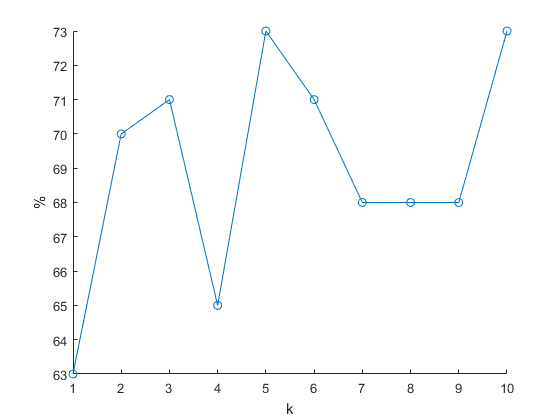
\includegraphics[width=\textwidth]{k_plot.png}
\caption{Wykres gęstości od liczby rozgałęzień}
\end{figure}

\item Funkcja minimalizująca wysokość

Gęstość dla $k=3$: 71

Najlepsza gęstość dla $k=10$: 75

Funkcja wysokości, nie najlepiej sprawdzająca się w większości przypadków, przy wąskiej studni radzi sobie porównywalnie z pozostałymi.

\item Funkcja maksymalizująca przyleganie

Gęstość dla $k=3$: 70

Najlepsza gęstość dla $k=7$: 76

Jest to najlepsza funkcja dla tego przypadku - dobry rezultat udało się osiągnąć przy stosunkowo małej wartości k.
\end{enumerate}
\subsubsection{Szerokość studni: 20}
Szerokość 20 jest najlepsza do porównania funkcji kosztu, a także zaobserwowania ich szczególnych cech.
Pozwala na większą swobodę ułożenia klocków niż szerokość 5, a jednocześnie wynikowa wysokość jest na tyle duża, że nierówności na górze nie mają istotnego wpływu na gęstość.
\begin{enumerate}
\item Funkcja minimalizująca dziury

Gęstość dla $k=3$: 75

Najlepsza gęstość dla $k=9$: 80

Na rysunku można zaobserwować pewną wadę tej funkcji - pozwala na tworzenie głębokich, wąskich dziur (jak na górze po lewej). 
Wynika to z tego, że takie zjawisko nie jest traktowane przez funkcję jako dziura.
Z kolei zakrycie takiej dziury klockiem znacząco zwiększa liczbę dziur, więc algorytm pozwoli na to tylko w ostateczności.

\begin{figure}[H]
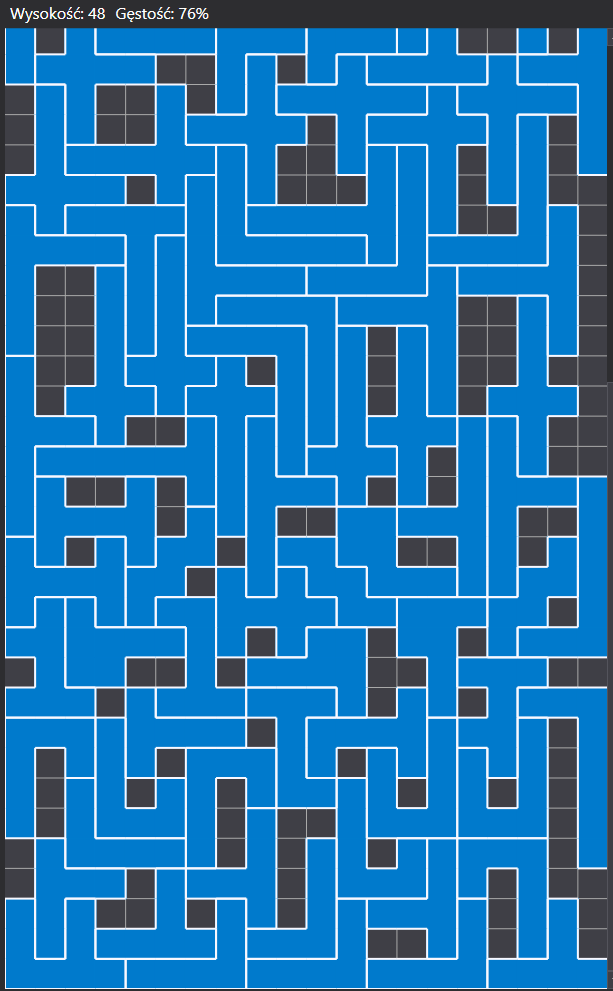
\includegraphics[width=\textwidth]{dziury.PNG}
\caption{Ułożenie klocków dla funkcji dziur}
\end{figure}

\item Funkcja minimalizująca wysokość

Gęstość dla $k=3$: 72

Najlepsza gęstość dla $k=10$: 76

W przypadku funkcji wysokości można zauważyć ciekawy wizualny efekt - klocki wydają się być położone maksymalnie pionowo.
Wynika to z faktu, że takie położenie minimalizuje wysokość w danym ruchu - nie ma znaczenia, że za kilka ruchów może się okazać niekorzystne.

\begin{figure}[H]
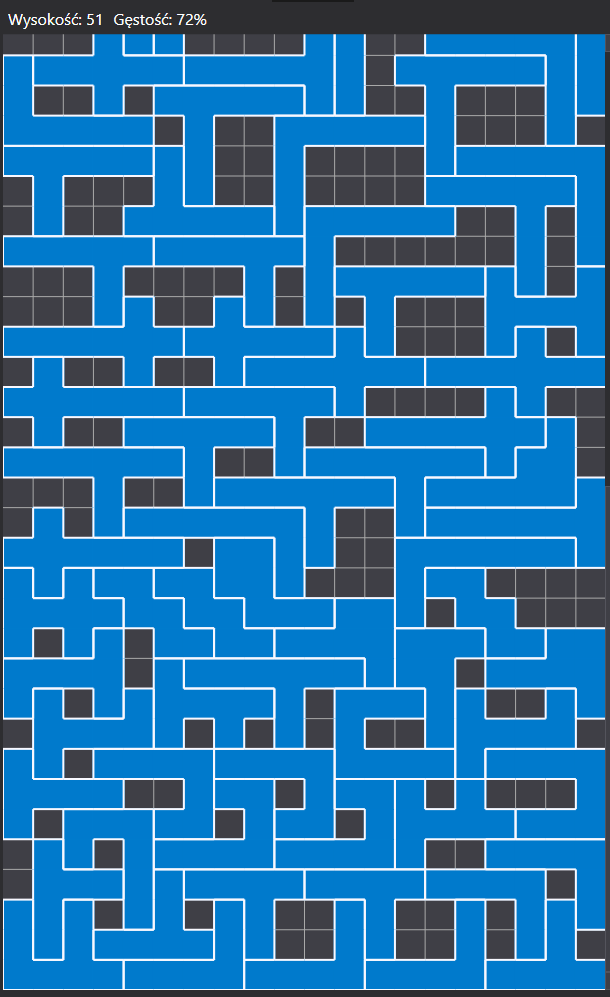
\includegraphics[width=\textwidth]{wysokosc.PNG}
\caption{Ułożenie klocków dla funkcji wysokości}
\end{figure}

\item Funkcja maksymalizująca przyleganie

Gęstość dla $k=3$: 76

Najlepsza gęstość dla $k=8$: 83

Funkcja przylegania sprawdziła się w tym przypadku najlepiej.

\begin{figure}[H]
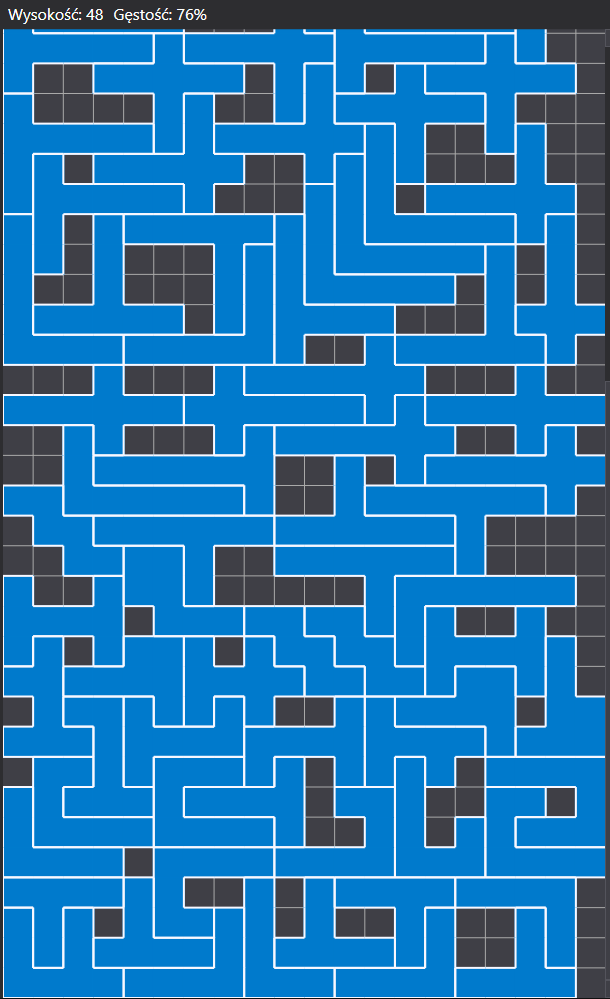
\includegraphics[width=\textwidth]{przyleglosc.PNG}
\caption{Ułożenie klocków dla funkcji przyległości}
\end{figure}

\end{enumerate}
\subsubsection{Szerokość studni: 80}
\begin{enumerate}

\item Funkcja minimalizująca dziury

Gęstość dla $k=3$: 66

Najlepsza gęstość dla $k=5$: 71

\begin{figure}[H]
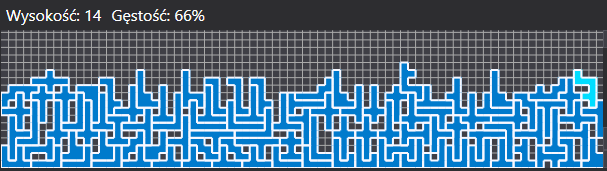
\includegraphics[width=\textwidth]{szeroka_plansza.PNG}
\caption{Ułożenie klocków dla funkcji przyległości}
\end{figure}

\item Funkcja minimalizująca wysokość

Gęstość dla $k=3$: 66

Najlepsza gęstość dla $k=9$: 66

\item Funkcja maksymalizująca przyleganie

Gęstość dla $k=3$: 66

Najlepsza gęstość dla $k=5$: 71

\end{enumerate}
\textbf{Wnioski}
W tym teście najlepsza okazała się funkcja przylegania, jednak niewiele tylko wyprzedziła funkcję dziur.

Warto zauważyć, że algorytm daje najlepsze wyniki dla średniej szerokości studni, co zgadza się z intuicją.
W przypadku małej szerokości, porównywalnej z szerokością niektórych klocków trudno jest osiągnąć dobre zapełnienie dziur - w niektórych momentach konieczne jest praktycznie układanie klocków jeden na drugim.
Z kolei przy szerokiej studni na wynik niekorzystnie wpływają górne mało zapełnione wiersze.
%\subsection{zestaw drugi...}
\section{Wnioski} %z testów
\end{document}